\documentclass{article}

\usepackage{amsmath, amssymb, amsfonts}
\usepackage{amsthm}
\usepackage{tikz}
\usepackage{thmtools}
\usepackage{graphicx}
\usepackage{setspace}
\usepackage{geometry}
\usepackage{float}
\usepackage{hyperref}
\usepackage[utf8]{inputenc}
\usepackage[english]{babel}
\usepackage{framed}
\usepackage{tcolorbox}
\usepackage{comment}
\usepackage{titlesec}
\usepackage{enumitem}
\usepackage{array}
\usepackage{multirow, bigdelim}
\usepackage{marginnote}
\usepackage{lipsum}
\usepackage{neuralnetwork}
\usepackage{subfigure}
\usepackage{slashed}
\usepackage{listings}
\usepackage{multicol}
\usepackage{mdframed}
\usepackage{listings}

\usetikzlibrary{graphs}
\usetikzlibrary{shapes}
\usetikzlibrary{backgrounds}
\usetikzlibrary{calc}
\usetikzlibrary{patterns}
\usetikzlibrary{positioning, fit, arrows.meta}

\newenvironment{solution}{\textit{Solution}.}

\titleformat{\subsection}[block]{\normalfont\Large\bfseries}{\thesubsection}{1em}{}
\titleformat{\subsubsection}[hang]{\normalfont\bfseries}{}{1em}{}

\colorlet{LightGray}{black!30}
\colorlet{LightOrange}{orange!15}
\colorlet{LightGreen}{green!15}
\colorlet{Orange}{orange!5}
\colorlet{LightRed}{red!50}
\colorlet{LightBlue}{blue!15}
\colorlet{Yellow}{yellow!50}
\colorlet{Red}{red!5}

\newcommand{\HRule}[1]{\rule{\linewidth}{#1}}


\lstdefinestyle{mystyle}{
    basicstyle=\ttfamily\upshape, % upshape for non-italic
    keywordstyle=\color{blue},
    language=Python,
    breaklines=true,
    mathescape=true,
}

\lstset{style=mystyle}


%%% Problem Numbering and Formatting

% Define a new style
\newtheoremstyle{upright}% name of the style
  {3pt}% Space above
  {3pt}% Space below
  {\upshape}% Body font: upright text
  {}% Indent amount
  {\bfseries}% Theorem head font: bold
  {.}% Punctuation after theorem head
  {.5em}% Space after theorem head
  {}% Theorem head spec (can be left empty, meaning ‘normal’)

% Apply the style to the 'problem' environment
\theoremstyle{upright}
\newtheorem{problem}{Problem}


\setstretch{1.2}
\geometry{
    textheight=9in,
    textwidth=5.5in,
    top=1in,
    headheight=12pt,
    headsep=25pt,
    footskip=30pt
}

\def \proofDistance {5pt}
\def \subheaderSpace {10pt}

\newcommand{\proofseparator}{\par\noindent\rule{\textwidth}{0.4pt}}
\newcommand{\caution}{\marginnote{
\includegraphics[width=2em]{caution.png}}}

% Natural Numbers 
\newcommand{\N}{\ensuremath{\mathbb{N}}}

% Whole Numbers
\newcommand{\W}{\ensuremath{\mathbb{W}}}

% Integers
\newcommand{\Z}{\ensuremath{\mathbb{Z}}}

% Rational Numbers
\newcommand{\Q}{\ensuremath{\mathbb{Q}}}

% Real Numbers
\newcommand{\R}{\ensuremath{\mathbb{R}}}

% Complex Numbers
\newcommand{\C}{\ensuremath{\mathbb{C}}}

\newmdenv[
  topline=false,
  bottomline=false,
  rightline=false,
  leftline=true,
  linewidth=1.5pt,
  linecolor=black, % default color, will be overridden in custom commands
  innertopmargin=0pt,
  innerbottommargin=0pt,
  innerrightmargin=10pt,
  innerleftmargin=10pt,
  leftmargin=0pt,
  rightmargin=0pt,
  skipabove=\topsep,
  skipbelow=\topsep
]{customframedproof}


% Command for problem statement
\newcommand{\pb}[1]{
    \begin{problem}
    #1
    \end{problem}
}

% Define a command for custom proofs with separator
\newcommand{\pf}[1]{
    \vspace{\proofDistance}
    \begin{proof}
    #1
    \end{proof}
    \proofseparator
}

\newcommand{\sol}[1]{
    \vspace{\proofDistance}
    \begin{customframedproof}
        \begin{solution}
        #1
        \end{solution}
    \end{customframedproof}
    \proofseparator
}

\newcommand{\solex}[1]{
    \vspace{\proofDistance}
    \begin{solution}
    #1
    \end{solution}
}

\renewcommand{\labelenumi}{(\alph{enumi})} % Changes the first level


\lstset{
    basicstyle=\ttfamily,
    keywordstyle=\color{blue},
    language=Python,
    breaklines=true,
    mathescape=true,
}

\begin{document}

\begin{center}
    \textbf{Practice Set VIII} \\
    
    \textbf{Name}: Paul Beggs \\
\end{center}

\pb{
You are given a list \texttt{lst} of distinct integers, $\texttt{lst} = \texttt{[}x_0,x_1,\dots x_{n-1}\texttt{]}$, which has length $n$ which is at least 2.
\begin{enumerate}
    \item (4 points) Write (in pseudocode) an algorithm which will return the \textit{second} largest value in the list. For example: \begin{itemize}
        \item if \texttt{lst} $=$ \texttt{[3, 6, 1, 4, 2]} your algorithm should return \texttt{4}
        \item if \texttt{lst} $=$ \texttt{[-3, -1, -6, -7]} your algorithm should return \texttt{-3}
    \end{itemize}
\end{enumerate}
}

    \vspace{0.5cm}

\begin{lstlisting}
    def find_second_largest(lst) -> int:
        if len(lst) < 2: # Check length - O(1)
            return None
            
        # Initial comparison and assignments - O(1)
        if lst[0] > lst[1]:
            maximum, 2nd_max = lst[0], lst[1]
        else:
            maximum, 2nd_max = lst[1], lst[0]
            
        # Loop through remaining elements - O(n-2)
        for num in lst[2:]:
        
            # Comparison to find new maximum or second maximum O(1)
            if num > maximum:
                2nd_max = maximum 
                maximum = num  
            elif num > 2nd_max:
                2nd_max = num  
        return 2nd_max
\end{lstlisting}

    
    \vspace{1cm}

\begin{enumerate}
    \setcounter{enumi}{1}
    \item (2 points) For your algorithm, determinimume a big-$\Theta$ estimate for the time complexity, in terms of $n$.
    \sol{
    $\Theta(n)$
    }
\end{enumerate}

\newpage

\pb{
You are given a list \texttt{lst} of distinct integers, $\texttt{lst} = \texttt{[}x_0,x_1,\dots x_{n-1}\texttt{]}$, which has length $n$ which is at least 2.
\begin{enumerate}
    \item (4 points) Write (in pseudocode) an algorithm which will return the largest product of a pair of distinct positions from the list. For example: \begin{itemize}
        \item if \texttt{lst} $=$ \texttt{[3, 6, 1, 4, 2]} your algorithm should return \texttt{24}
        \item if \texttt{lst} $=$ \texttt{[-3, -1, -6, -7]} your algorithm should return \texttt{42}
    \end{itemize}
\end{enumerate}
}
\vspace*{\fill}
\begin{lstlisting}
    def maximum_pair_product(lst) -> int:
        # Initialize the largest and second largest - O(1)
        if lst[0] > lst[1]:
            maximum, 2nd_max = lst[0], lst[1]
        else:
            maximum, 2nd_max = lst[1], lst[0]
    
        # Initialize the smallest and second smallest - O(1)
        if lst[0] < lst[1]:
            minimum, 2nd_min = lst[0], lst[1]
        else:
            minimum, 2nd_min = lst[1], lst[0]
    
        # Traverse through the list starting from the third element - O(n-2)
        for num in lst[2:]:
            if num > maximum:
                2nd_max = maximum 
                maximum = num
            elif num > 2nd_max:
                2nd_max = num  
    
            if num < minimum:
                2nd_min = minimum 
                minimum = num 
            elif num < 2nd_min:
                2nd_min = num 
        return max(maximum * 2nd_max, minimum * 2nd_min)
\end{lstlisting}
\vspace{0.5cm}
\begin{enumerate}
    \setcounter{enumi}{1}
    \item (2 points) For your algorithm, determinimume a big-$\Theta$ estimate for the time complexity, in terms of $n$.
    \sol{
    $\Theta(n)$
    }
\end{enumerate}

\newpage

\pb{
(3 points each) For each graph shown, use Prim's Algorithm to determine a minimal weight spanning tree. For each, list the total weight of the tree you find.
}
\begin{enumerate}
    \item $V = \{h,a,d,b,c,e,j,i,g,f\}$; $E = \{3,2,1,2,2,2,3,2,3\} = 20$ -- Total weight


\begin{figure}[htbp]
    \centering
    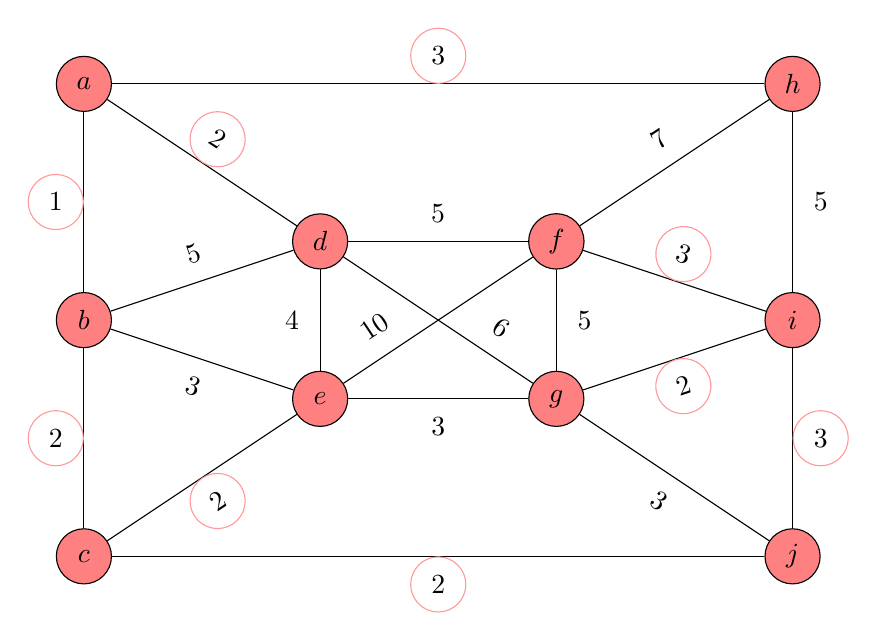
\begin{tikzpicture}[every node/.style={circle, draw, minimum size=0.7cm}, scale=1]
        \node[fill=red!50] (c) at (0,0) {$c$};
        \node[fill=red!50] (a) at (0,6) {$a$};
        \node[fill=red!50] (j) at (9,0) {$j$};
        \node[fill=red!50] (h) at (9,6) {$h$};

        \node[fill=red!50] (e) at (3,2) {$e$};
        \node[fill=red!50] (d) at (3,4) {$d$};
        \node[fill=red!50] (g) at (6,2) {$g$};
        \node[fill=red!50] (f) at (6,4) {$f$};

        \node[fill=red!50] (b) at (0,3) {$b$};
        \node[fill=red!50] (i) at (9,3) {$i$};



        % Rectangle parameter
        \draw (c) -- node [midway, below, draw=red!40] {2} (j);
        \draw (c) -- node [midway, left, draw=red!40] {2} (b);
        
        \draw (a) -- node [midway, above, draw=red!40] {3} (h);
        \draw (a) -- node [midway, left, draw=red!40] {1} (b);

        \draw (h) -- node [midway, right, draw=none] {5} (i);
        
        \draw (j) -- node [midway, right, draw=red!40] {3} (i);

        % Inner square
        \draw (d) -- node [pos=0.75, above, sloped, draw=none] {6} (g);
        \draw (f) -- node [pos=0.75, above, sloped, draw=none] {10} (e);

        \draw (g) -- node [midway, right, draw=none] {5} (f);
        \draw (e) -- node [midway, left, draw=none] {4} (d);  
        
        % X
        \draw (d) -- node [midway, above, draw=none] {5} (f);
        \draw (g) -- node [midway, below, draw=none] {3} (e);

        % Inner triangles
        \draw (d) -- node [midway, above, sloped, draw=none] {5} (b);
        \draw (e) -- node [midway, below, sloped, draw=none] {3} (b);

        \draw (c) -- node [midway, below, sloped, draw=red!40] {2} (e);
        \draw (a) -- node [midway, above, sloped, draw=red!40] {2} (d);

        \draw (g) -- node [midway, below, sloped, draw=none] {3} (j);
        \draw (g) -- node [midway, below, sloped, draw=red!40] {2} (i);

        \draw (f) -- node [midway, above, sloped, draw=red!40] {3} (i);
        \draw (f) -- node [midway, above, sloped, draw=none] {7} (h);
    \end{tikzpicture}
\end{figure}

\item $V = \{b,c,f,j,e,a,d,h,k,l,m\}$; $E = \{1,2,5,2,3,3,2,3,3,2,2\} = 28$ -- Total weight
\begin{figure}[htbp]
    \centering
    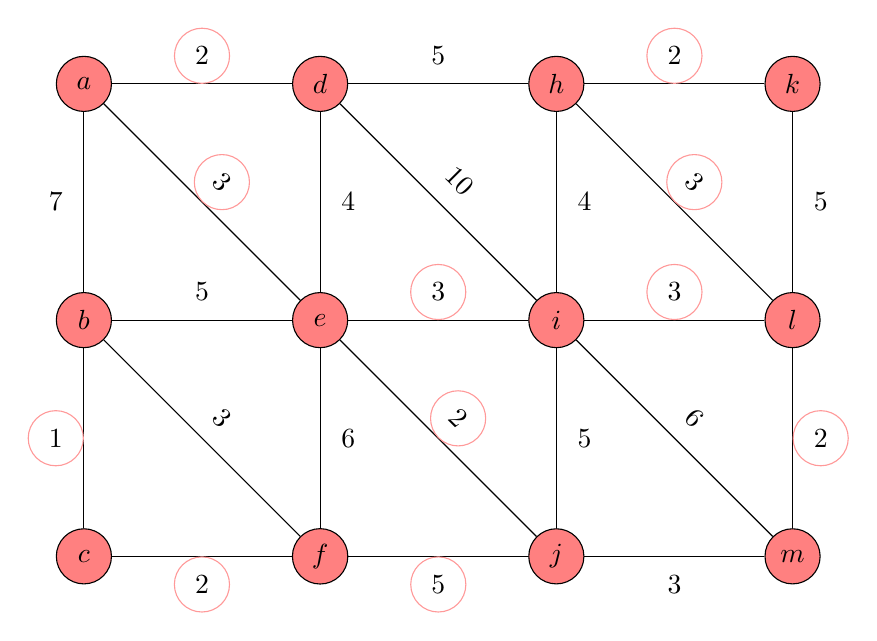
\begin{tikzpicture}[every node/.style={circle, draw, minimum size=0.7cm}, scale=1]
        \node[fill=red!50] (c) at (0,0) {$c$};
        \node[fill=red!50] (a) at (0,6) {$a$};
        \node[fill=red!50] (m) at (9,0) {$m$};
        \node[fill=red!50] (k) at (9,6) {$k$};

        \node[fill=red!50] (b) at (0,3) {$b$};
        \node[fill=red!50] (l) at (9,3) {$l$};

        \node[fill=red!50] (f) at (3,0) {$f$};
        \node[fill=red!50] (j) at (6,0) {$j$};

        \node[fill=red!50] (e) at (3,3) {$e$};
        \node[fill=red!50] (i) at (6,3) {$i$};

        \node[fill=red!50] (d) at (3,6) {$d$};
        \node[fill=red!50] (h) at (6,6) {$h$};


        % Parameter
        \draw (a) -- node [midway, left, draw=none] {7} (b);
        \draw (b) -- node [midway, left, draw=red!40] {1} (c);

        \draw (k) -- node [midway, right, draw=none] {5} (l);
        \draw (l) -- node [midway, right, draw=red!40] {2} (m);

        % Flooring
        \draw (c) -- node [midway, below, draw=red!40] {2} (f);
        \draw (j) -- node [midway, below, draw=red!40] {5} (f);
        \draw (j) -- node [midway, below, draw=none] {3} (m);

        \draw (e) -- node [midway, above, draw=none] {5} (b);
        \draw (e) -- node [midway, above, draw=red!40] {3} (i);
        \draw (l) -- node [midway, above, draw=red!40] {3} (i);

        \draw (d) -- node [midway, above, draw=red!40] {2} (a);
        \draw (d) -- node [midway, above, draw=none] {5} (h);
        \draw (k) -- node [midway, above, draw=red!40] {2} (h);

        % Walls
        \draw (e) -- node [midway, right, draw=none] {4} (d);
        \draw (e) -- node [midway, right, draw=none] {6} (f);

        \draw (i) -- node [midway, right, draw=none] {4} (h);
        \draw (i) -- node [midway, right, draw=none] {5} (j);

        % Diagonals
        \draw (e) -- node [midway, above, sloped, draw=red!40] {3} (a);
        \draw (e) -- node [midway, above, sloped, draw=red!40] {2} (j);

        \draw (b) -- node [midway, above, sloped, draw=none] {3} (f);

        \draw (h) -- node [midway, above, sloped, draw=red!40] {3} (l);

        \draw (i) -- node [midway, above, sloped, draw=none] {10} (d);
        \draw (i) -- node [midway, above, sloped, draw=none] {6} (m);
    \end{tikzpicture}
\end{figure}
\end{enumerate}

\newpage

\pb{
Consider the list, $[7,2,4,9,1,5,13,12,3,8]$.
}
\begin{enumerate}
    \item (2 points) Construct a binary search tree for this list, using 7 as the root (i.e., do not try to rebalance!)

    \begin{figure}[htbp]
        \centering
        \begin{tikzpicture}[level/.style={sibling distance=60mm/#1}]
            \node [circle, draw] (z){$7$}
            child {node [circle, draw] (a) {$2$}
                child {node [circle, draw] (b) {$1$}}
                child {node [circle, draw] (c) {$4$}
                    child {node [circle, draw] (d) {$3$}}
                    child {node [circle, draw] (e) {$5$}}
                }
            }
            child {node [circle, draw] {$9$}
                child {node [circle, draw] {$8$}}
                child {node [circle, draw] {$13$}
                    child {node [circle, draw] {$12$}}
                    child {node [circle] {$\quad$} edge from parent[draw=none]} % null drawings to align the tree placement
                }
            };
        \end{tikzpicture}
    
    \end{figure}
    
    \item (2 points) In what order are the nodes visited by a preorder traversal?
    \sol{$\{7,2,1,4,3,5,9,8,13,12\}$}
    \item (2 points) In what order are the nodes visited by a postorder traversal?
    \sol{$\{1,3,5,4,2,8,12,13,9,7\}$}
    \item (2 points) In what order are the nodes visited by a inorder traversal?
    \sol{$\{1,2,3,4,5,7,8,9,12,13\}$}
\end{enumerate}

\end{document}